% $Id: elliptic.tex,v 1.1 1992/02/24 01:01:16 rz Exp rz $
\chapter{Elliptic Curves}
\label{Elliptic:Chap}

\def\sumonlattice#1#2{\sum_{\scriptstyle#1 \in #2 \atop\scriptstyle #1 \not=0}}

In many complicated problems, especially those related to factoring
integers and proving the primality of integers, we study the structure
of certain finite groups.  For instance, to prove that $N$ is a prime
we examine the set of integers modulo $N$ and attempt to prove that
they form a group of order $\phi(N)= N-1$.  This is most easily done
by exhibiting an integer whose multiplicative order modulo $N$ is $N-1$.
Ultimately, this requires factoring $N-1$, which we hope is easy.
However, this is not always the case.

Many of these algorithms can be saved by using elliptic curves instead
of the set of points modulo $N$.  Consider the equation 
\[
E: y^2 = 4x^3 - a x - b,
\]
where $a$ and $b$ are fixed parameters related to $N$.  Denote by
$N_p(E)$ the number of zeroes of $E$ in the finite field $\F_p$.  Of
the $p^2$ candidates we would expect there to be $O(p)$ zeroes.  In
fact,
\begin{equation}\label{Ell:Simp:RH:Eq}
p - 2 \sqrt{p} \le N_p(E) \le p + 2 \sqrt{p}.
\end{equation}
Furthermore, the zeroes of $E$ possess a group structure.

While the straightforward algorithms use the group of integers modulo
$N$, with the elliptic curve versions we can choose from a set of
groups by varying $a$, $b$ and $p$.  So instead of having a single
group of order $N-1$ to work with we can choose from a set of groups
of varying sizes.  This additional flexibility makes elliptic curves
extremely powerful tools in complexity theory.

The theory of elliptic curves is one of the fields of mathematics that
lies on the crack between several different fields: analysis, geometry
and number theory.  The interaction between these fields leads to some
very beautiful and deep theorems.  In this section we will only touch
on a few high points.  It also means that there are many different
ways of approaching each definition and theorem in the field.  A text
on elliptic curves written from an analytic viewpoint is almost
unintelligible to one only familiar with the algebraic viewpoint.  In
this chapter we have tried to use the most direct techniques available
concomitant with using as little machinery as possible.  Nonetheless,
we use a number of terms that are not fully defined until
\chapref{Geometry:Chap}.  

\medskip

\index{point on a curve} \index{curve} \index{elliptic curve}
\index{Weierstrass normal form}
Let $k$ be a field and $f(x,y)$ a polynomial with coefficients in $k$.
The set of all pairs $(x_0, y_0)$ were each coordinate is in $k$ and where
$f(x_0,y_0) = 0$ is called a {\em curve} and the pair $(x_0,y_0)$ is
called a {\em point on the curve\/}.  $f(x, y) = 0$ is called the
defining equation of the curve.  Elliptic curves have defining equations
of degree three.  In general they satisfy an equation of the form
\[
y^2 + a_1 x y + a_3 y = x^3 + a_2 x^2 + a_4 x + a_6.
\]
If the characteristic of $k$ is not $2$ or $3$, then a
suitable substitution transforms this equation into the
{\em Weierstrass normal form\/}:\index{elliptic curve! Weierstrass
normal form}
\[
y^2 = x^3 + A x + B.
\]

The set of points on an elliptic curve form a group, and it is this
group that we use to solve several computational number theory
problems.  To motivate the organization of this group we begin by
discussing a simpler group based on the quadratic equation in
\sectref{Circle:Group:Sec}.  We then introduce elliptic curves in
\sectref{Elliptic:Intro:Sec}, the group law on elliptic curves in
\sectref{Elliptic:Addition:Sec} and the ring of endomorphisms of an
elliptic curve in \sectref{Elliptic:Endo:Sec}.
\sectref{Elliptic:Zeta:Sec} introduces the zeta function of an
elliptic curve and relates it to the Riemann zeta function discussed
in \sectref{Prime:Dist:Sec}.  Finally, a technique for computing the
order of additive group is presented in \sectref{Elliptic:Order:Sec}.

\section{The Circle Group}
\label{Circle:Group:Sec}

\begin{figure}
\begin{center}
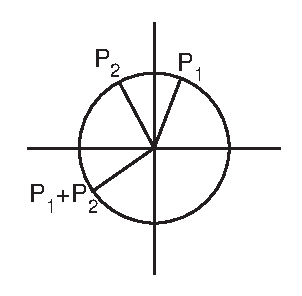
\includegraphics{CircleGroup}
\end{center}
\caption{Addition of Two points in the Circle Group\label{Circle:Group:Fig}}
\end{figure}

Consider the curve with defining equation $x^2 + y^2 =1$.  Its image
in the real plane is a circle.  In this section we show how to define
an abelian group structure on the points of the of the curve.  Let
$P_1 = (x_1, y_1)$ and $P_2 = (x_2, y_2)$ be two such points, as show
in \figref{Circle:Group:Fig}.  Therefore we have $x_1^2 + y_1^2 = 1$
and $x_2^2 + y_2^2 = 1$.  Looking at the image in the real plane, we
define their sum to be the point whose angle with real axis is the sum
of the angles of $P_1$ and $P_2$.  That is,
\begin{eqnarray*}
P_1 + P_2 = P_3 &= &
(\cos (\arctan {\frac{y_1}{x_1}} + \arctan {\frac{y_2}{x_2|}}),\,
\sin (\arctan {\frac{y_1}{x_1}} + \arctan {\frac{y_2}{x_2}}))\\
&=& (x_1 x_2 - y_1 y_2, x_1 y_2 + y_1 x_2).
\end{eqnarray*}
The definition using sines and cosines is based on our geometrical
intuition about the circle.  However the algebraic definition is a
natural generalization and more widely applicable, The identity element
of this operation is the point $(1, 0)$.  If $P_1$ and $P_2$ lie on the
unit circle, $P_3$ is also on the unit circle.  It is easy to see that
the points on the unit circle for a group using this addition law.

More generally, if $R$ is any commutative ring with unit, and $G$ those
elements $(x, y) \in R \times R$ such that $x^2 + y^2 = 1$, then we can
make $G$ into a group by formally using the group law
\[
(x_1, y_1) + (x_2, y_2) = (x_1 x_2 - y_1 y_2, x_1 y_2 + y_1 x_2).
\]
Each of the group axioms can be verified formally.  For instance, $G$ is
closed under addition since
\[
(x_1 x_2 - y_1 y_2)^2 + (x_1 y_2 + x_2 y_1)^2 
= (x_1^2 + y_1^2) (x_2^2 + y_2^2).
\]

We denote by $C_p$ the group defined by this law for $R = \F_p$.  How
many elements are there in $C_p$?  That is, how many solutions are
there of $x^2 + y^2 =1$ in $\F_p \times \F_p$?  One way to look at
this is to examine the partitions of $1 = a + b$ where $a, b \in
\F_p$.  This is easy to compute.  There are $p$ such partitions.  Then
we need to count the number of solutions of $x^2 = a$ and $y^2 = b$
there are in $\F_p$.  As pointed out in \propref{NumQuadSol:Prop}, the
number of solutions of $x^2 = a$ is $1 + (a/p)$.  So the number of
elements in $C_p$ is
\begin{eqnarray*}
\# C_p &=& \sum_{\scriptstyle a + b = 1 \atop \scriptstyle a, b
\in \F_p}
\left( 1 + \left(\frac{a}{p} \right) \right)
\left( 1 + \left(\frac{b}{p} \right) \right) \\
&= &p + \sum_{a \in \F_p} \left(\frac{a}{p} \right)
+ \sum_{b \in \F_p} \left(\frac{b}{p} \right)
+ \sum_{\scriptstyle a + b = 1 \atop \scriptstyle a, b \in \F_p}
\left(\frac{a}{p} \right) \left(\frac{b}{p} \right).
\end{eqnarray*}
The first two sums are zero.  The third sum is not hard to evaluate.
The quadratic character of $b$ is the same as that of $1/b$.  Therefore
we have
\begin{eqnarray*}
\sum_{\scriptstyle a + b = 1 \atop \scriptstyle a, b \in \F_p}
\left(\frac{a}{p} \right) \left(\frac{b}{p} \right) &= &
\sum_{\scriptstyle a + b = 1 \atop \scriptstyle b \not= 0}
\left(\frac{a}{p} \right) \left(\frac{1/b}{p} \right) = 
\sum_{\scriptstyle a + b = 1 \atop \scriptstyle b \not= 0}
\left(\frac{a/b}{p} \right)\\
&=& \sum_{a \not= 1} \left(\frac{a/(1- a)}{p }\right).
\end{eqnarray*}
Since $a/(1- a)$ is an invertible bilinear transformation, we can replace
$a/(1- a)$ by $c$.  The constraint that $a\not= 1$ translates to
$c\not= -1$.
\[
\# C_p = p + \sum_{c \not = -1} \left(\frac{c}{p} \right) 
= p - \left(\frac{-1}{p}\right) = p - (-1)^{\frac{p -1}{2}},
\]
where we have used \propref{FF:Euler:Residue:Prop} to evaluate the
last Jacobi symbol.  Thus when $p \equiv 3 \pmod 4$, $C_p$ has $p+1$
elements.  Otherwise $C_p$ has $p-1$ elements.

\medskip
There is a correspondence between the points of the circle group with
real coordinates and the points in the plane. The solution to $x^2 + y^2
= 1$ can be parameterized as
\begin{eqnarray*}
y(\theta) &= &\sin(\theta),\\
x(\theta) &= &\cos(\theta) = \frac{d}{d\theta} y(\theta).
\end{eqnarray*}
The addition formula was set up so that if
$P_i = (x(\theta_i), y(\theta_i))$ and
$P_1 + P_2 = P_3$, then $\theta_1 + \theta_2 = \theta_3$.
Notice that we could express $x(\theta)$ as the derivative of
$y(\theta)$, so $y(\theta)$ is a solution of the differential equation
\[
Y'^2 = 1 -y^2.
\]

The sine function is periodic with period $2\pi$.  We view $y(\theta)$
as a function of a complex variable.  The period of $y$ defines a one
dimensional lattice in the complex plane,
\[
L_1 = \{ \ldots, -2\pi, 0, 2\pi, 4\pi, \ldots \}.
\]
The parameterization function $y(\theta)$ defines a one to
one correspondence between $\C / L_i$ and the circle.  Addition on the
quadratic curve corresponds to addition of complex numbers in the
$\theta$ plane.

We summarize these results as follows
\begin {itemize}
\item over the reals there is a one to one correspondence
\[
x^2 + y^2 = 1 \Longleftrightarrow \R/\Z
\]
induced by $(x, y) = (\sin \theta, \cos \theta)$.

\item  Over the finite field $\F_p$, the points on the curve $C_p : x^2+y^2=1$
form a group which arises from the correspondence with $\R/\Z$.

\item The number of points elements of $C_p$ is $p \pm 1$ which we can
write as
\[
\left| N_p(C_p) - p \right| = 1.
\]
\end{itemize}

\section{Introduction to Elliptic Curves}
\label{Elliptic:Intro:Sec}

In this section we carry over the ideas from the circle group to
elliptic curves.  The approach we use is to replace the one
dimensional lattice $\Z$ by a two dimensional lattice, $L$, in the
complex plane.  $\C/L$ plays the role of the circle $\R/\Z$.
It also has an abelian group structure under addition. 

To create the desired algebraic structure we build a function $f(z)$
over the complex plane, that is periodic modulo $L$, and then show
that $f(z)$ and $f'(z)$ satisfy a {\em polynomial} identity $P(f, f')
= 0$.  $P$ will provide the isomorphism between the algebraic
curve\index{algebraic curve} $P(x, y) = 0$ and the additive group
$\C/L$.  We can then use the points of the algebraic curve $P(x, y) =
0$, reduced modulo a prime, as a finite group for other calculations. 

Let $L \subset \C$ be a two dimensional lattice generated by the two
linearly independent complex numbers $\omega_1$ and $\omega_2$.  The
ratio of the two periods $\omega_1/\omega_2$ is be a complex number.
For a fixed complex number $z$, the set of all points $z + t_1
\omega_1 + t_2 \omega_2$ with  $0 \le t_i < 1$ is called a \keyi{fundamental
parallelogram} of $L$.  If $S$ is a fundamental parallelogram of $L$,
then every point in $\C$ is equivalent, modulo $L$, to some point in
$S$.  
 
The primitive function used in the circle case is $\sin \pi z$ (if we
normalize the period to be $1$).  The most direct relation between the
lattice points, $\Z$, and $\sin \pi z$ is the infinite product
\begin{equation}\label{Ell:Sin:Prod:Eq}
\sin \pi z = 
\pi z \prod^{\infty}_{\ell=1}\left(1 - \frac{z^2}{\ell^2}\right).
\end{equation}
This sum can be interpreted as a better (\ie{} convergent) way to
write
\[
\prod_{\ell \in \Z}(z - \ell),
\]
which vanishes at all of the zeroes of $\sin \pi z$.  However, to make
the two dimensional generalization, a different form is necessary.
Taking the logarithm of both sides of \eqnref{Ell:Sin:Prod:Eq} and
then differentiating we have 
\[
\begin{aligned}
\pi \cot \pi z & = \frac{1}{z} + 
\sum_{\ell = 1}^{\infty} \frac{2z}{z^2 - \ell^2}, \\
& = \frac{1}{z}
\sum_{\ell = 1}^{\infty} \frac{1}{z + \ell} + \frac{1}{z - \ell}, \\
& = \frac{1}{z}
\sum_{\ell = 1}^{\infty} 
 \left(\frac{1}{z + \ell} - \frac{1}{\ell}\right)
 +\left(\frac{1}{z - \ell} + \frac{1}{\ell}\right).
\end{aligned}
\]
The extra $1/\ell$ term is introduced makes the series generated by
the terms in parentheses absolutely convergent.  Rearranging the terms
we have
\begin{equation} \label{Ell:Cot:Sum:Eq}
\pi \cot \pi z = \frac{1}{z} +
{\sum_{\ell \in \Z}}'\left(\frac{1}{z - \ell} + \frac{1}{\ell}\right).
\end{equation}
Here, and in the future, we have used $\sum'$ to indicate that the sum
omits the $\ell = 0$ case.

Notice that $\pi \cot \pi x$ is is periodic with period $1$, a fact
that is not obvious from \eqnref{Ell:Cot:Sum:Eq}.  Simply replacing
$\Z$ in \eqnref{Ell:Cot:Sum:Eq} by the two dimensional lattice
\begin{equation}\label{Ell:Lat:Div:Eq}  
f(z)= \frac{1}{z} + \sum_{\ell \in L}' \frac{z}{\ell(z - \ell)}
\end{equation}
is not adequate.  The number of points in $L$ with absolute value
between $N-\frac{1}{2}$ and $N+\frac{1}{2}$ is $O(N)$.  Adding up the
terms in the annulus $N-\frac{1}{2} < \ell \le N+\frac{1}{2}$ gives
\[
\left| \sum_{N-\frac{1}{2} < \ell \le N+\frac{1}{2}}\frac{z}{\ell(z -
\ell)} \right|
\approx \frac{z}{z - N}
\]
so \eqnref{Ell:Lat:Div:Eq} diverges.  This can be fixed by defining the
function $\wp(z)$ to be 
\[
\wp(z) = \frac{1}{z^2} + 
{\sum_{\ell \in L}}' \frac{1}{(z - \ell)^2} - \frac{1}{\ell^2}.
\]
Since $-\ell$ is an element of $L$ if $\ell$ is, $\wp(z)$ must be an
even function.  However, it is not obvious that $\wp(z)$ is periodic.
Its derivative is
\[
\wp'(z) = -2 {\sum_{\ell \in L}}\frac{1}{(z - \ell)^3},
\]
which is clearly both odd and periodic.  Thus $\wp(z + \omega) = \wp(z) +
C$ where $\omega$ is a basis element of $L$ and $C$ is some constant.
Letting $z = - \omega/2$ we see that $C$ must be zero because $\wp(z)$
is even.  Thus $\wp(z)$ is also periodic.

Next we will show that $\wp(z)$ and $\wp'(z)$ are algebraically
dependent.  This is done by developing their power series expansions and
then looking for combinations that have no poles.  Since $\C/L$ is a
compact set, a function with no poles in $\C/L$ it must be zero.  Thus
we will not need to look at the entire power series expansions.

We can write
\begin{eqnarray*}
\frac{1}{(z-\ell)^2}- \frac{1}{\ell^2} &
=& \frac{2 z}{\ell^3} + \frac{3 z^2}{\ell^4} + \frac{4 z^3}{\ell^5} +
\cdots\\
&=& \sum_{n=1}^{\infty} \frac{(n+1)z^n}{\ell^{n+2}}.
\end{eqnarray*}
Using this in the definition of $\wp(z)$ gives
\[
\begin{aligned}
\wp(z) &=
\frac{1}{z^2} + {\sum_{\ell \in L}}'\sum_{n=1}^{\infty} \frac{(n+1)z^n}{\ell^{n+2}} \\
&= \frac{1}{z^2} + \sum_{n=1}^{\infty} (n+1) z^n 
\sumonlattice{\ell}{L} \frac{1}{\ell^{n+2}}\\
&= \frac{1}{z^2} + \sum_{n=1}^{\infty} (n+1) G_{n+2} z^n,
\end{aligned}
\]
where we have defined $G_k$ to be
\[
G_k = {\sum_{m,n \in \Z}}' \frac{1}{(m \omega_1 + n \omega_2)^k}.
\]
The $G_k$ are zero for odd $k$, since lattice points and their 
inverses will cancel each other.  Thus the first few terms of the power
series for $\wp(z)$ is
\[
\wp(z) = \frac{1}{z^2} + 3 G_4 z^2 + 5 G_6 z^4 + 7 G_8 z^6 + \cdots.
\]
Differentiating both sides of the equation gives
\[
\wp'(z) = -\frac{2}{z^3} + \frac{6 G_4}{z} + 20 G_6 z + 42 G_8 z^3 +
\cdots.
\]

These equations gives us enough information to find the polynomial
relationship between $\wp(z)$ and $\wp'(z)$.  For any polynomial
$f(x,y)$ then $f(\wp(z), \wp'(z))$ will be be an elliptic function.
Thus to prove that $f(\wp(z), \wp'(z))$ is zero we need only show that
it has less than 2 poles.  Since $\wp(z)$ has a pole of order $2$ and
$\wp'(z)$ one of order $3$, the smallest candidate polynomial must have
a $4x^3-y^2$ term.  Expanding this out we have
\begin{eqnarray*}
4\wp(z) - \wp'(z)^2 &=&
\frac{60 G_4}{z^2} + 140 G_6 + (72 G_4^2 + 252 G_8) z^2 \\
&&\qquad + (120 G_4 G_6 +396 G_{10})z^4 + \cdots.
\end{eqnarray*}
To cancel the next term we need only include a linear term in $x = \wp(z)$
\[
\begin{aligned}
4 \wp(z)^3 & - 60 G_4 \wp(z) - \wp'(z)^2 \\
 & = 140G_6 + (252 G_8 - 108 G_4^2) z^2 
     + (396 G_{10} - 180 G_6 G_4) z^4 + \cdots.
\end{aligned}
\]
Since this expression has no poles it must be a constant.  Thus, 
\[
\wp'(z)^2 = 4 \wp(z)^3 - 60 G_4 \wp(z) - 140 G_6.
\]
Furthermore, we can see that all $G_k$ for $k$ larger than 6 can be
determined from $G_4$ and $G_6$.  By these calculations we have
$G_8 = \frac{3}{7} G_4^2$ and $G_{10} = \frac{5}{11} G_4 G_6.$
In the literature, we frequently see this equation written as
\begin{equation} \label{Weier:DE:Eq}
\wp'(z)^2 = 4\wp(z)^3 -g_2 \wp(z) - g_3,
\end{equation}
where $g_2 = 60G_4$ and $g_3 = 140G_6$.

This relationship also gives us the one to one correspondence between
points in $\C/L$ and points on the elliptic curve 
$y^2 = 4 x^3 - g_2 x - g_3$.  Each point $(x,y)$ can be identified
with a complex number $z$ such that $x = \wp'(z)$ and $y = \wp(z)$.

\begin{proposition}
For each lattice $L$ in the complex plane, there exists a function
$\wp(z)$ such that $\wp(z + \ell) = \wp(z)$ if $\ell \in L$ and that
satisfies the differential equation
\[
\wp'(z)^2 = 4\wp(z)^3 -g_2 \wp(z) - g_3,
\]
\end{proposition}

\begin{figure}
\begin{center}
\begin {tabular}{ccc}
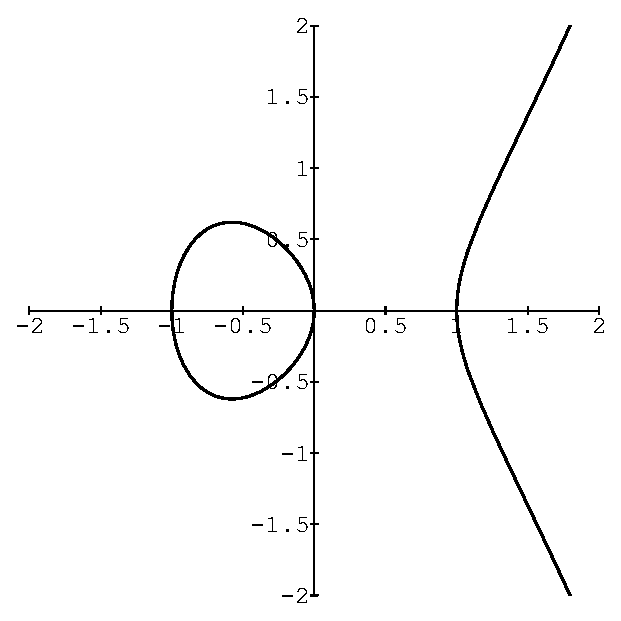
\includegraphics[width=1.3truein]{x3-x} &
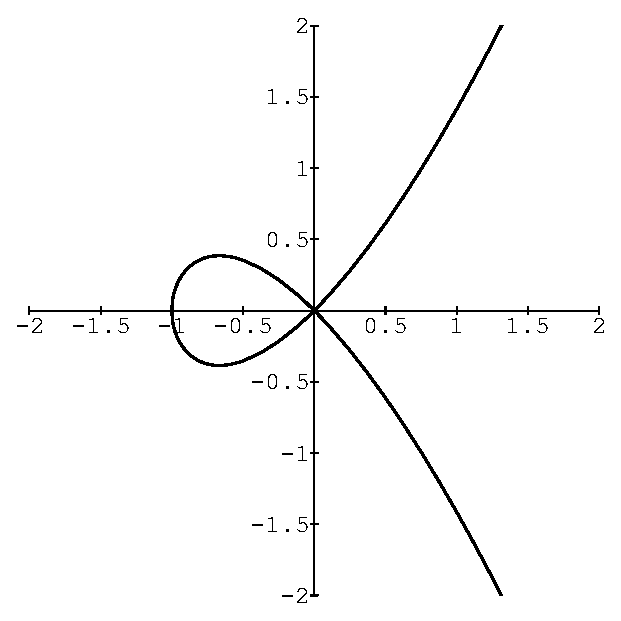
\includegraphics[width=1.3truein]{x3+x2} &  
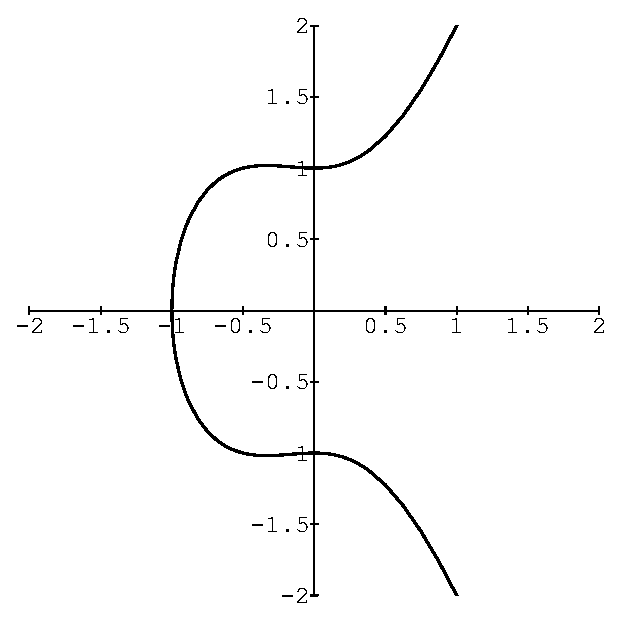
\includegraphics[width=1.3truein]{2x3+x2+1} \\
$y^2 = x^3 -x $ & $y^2=x^3+x^2$ & $y^2=2x^3+x^2+1$ 
\end{tabular}
\end{center}
\caption{Some Elliptic Curves}
\end{figure}

Thus  the elliptic curve that corresponds to the circle in
\sectref{Circle:Group:Sec} is
\begin {equation}\label{Ell:Weier:form:Eq}
E : y^2 = 4x^3 - g_2 x - g_3.
\end{equation}
The map
\[
z \longleftrightarrow (\wp(z), \wp'(z))
\]
provides a correspondence between $\C/L$ and the zeroes of
\eqnref{Ell:Weier:form:Eq}.  More precisely, if $P_i = (x_i, y_i)$ are
zeroes of \eqnref{Ell:Weier:form:Eq}, we want to define 
\[
P_1 + P_2 = ( \wp(\wp^{-1}(x_1) + \wp^{-1}(x_2)), 
\wp'(\wp^{-1}(x_1) + \wp^{-1}(x_2))).
\]
Thus the group structure the points on $E$ depends upon the addition
formula of $\wp$.  Fortunately, the addition formula for $\wp$ does
not involve any transcendental computations as shown in the next section.

\section{Addition Formulas on Elliptic Curves}
\label{Elliptic:Addition:Sec}

The points on an elliptic curve can be given the structure of an
abelian group similar to that of the points on the circle discussed in
\sectref{Circle:Group:Sec}.  However, the construction for elliptic
curves is somewhat more intricate than that for circles.  In this
section we develop this additive group in two different fashions.  
\sectref{Elliptic:WP:Add:Sec} constructs the additive group from a two
dimensional lattice in place of the one dimensional lattice used in
the case of the circle.  The Weierstrass $\wp$ function is used to tie
this abelian group to an elliptic curve in Weierstrass normal form. 
\sectref{Elliptic:Geo:Add:Sec} develops the group law using geometric
reasoning on the elliptic curve itself.  Finally Sections
\ref{Elliptic:Alg:Add:Sec} and \ref{Elliptic:Hessian:Add:Sec} give to
purely algebraic forms of the addition law, which can be used for
elliptic curves over fields of characteristic.

\subsection{Addition Formulas for $\wp$}
\label{Elliptic:WP:Add:Sec}

Let $f(x)$ a doubly periodic function, with periods $\omega_1$ and
$\omega_2$ that is meromorphic on $\C$ and thus $\C/L$.  Such a
function is called an elliptic function.  The line integral of $f$
around a fundamental parallelogram will be zero since the value on
opposite sides will be the same.  By Cauchy's theorem we have
\[
2 \pi i \sum \res f = \int_\Gamma f\,dz = 0,
\]
so the sum of the residues must be zero.  Consequently an elliptic
function must have at least two poles, counting multiplicities, within
the fundamental parallelogram.


Let $E$ be an elliptic curve with associated lattice $L$ as before.
Under addition the complex numbers are abelian group.  Since the sum of
two elements of $L$ is still in $L$ the additive group structure of $\C$
induces an abelian group structure on $\C/L$.  By the correspondence
given by the Weierstrass-$\wp$ function, this induces a group law on the
points of $E$.  Let $P_1 = (\wp(z_1), \wp'(z_1), 1)$ and 
$P_2 = (\wp(z_2), \wp'(z_2), 1)$ be two points on $E$ where 
$z_1$ and $z_2$ are elements of a fundamental parallelogram of $L$.  We
define the sum of $P_1$ and $P_2$ to be the point
$P_3 = (\wp(z_3), \wp'(z_3), 1)$ where 
$z_3 = z_1 + z_2 \pmod L$.  

This addition law can be expressed algebraically as a rational function in
the coordinates of $P_1$ and $P_2$.\Marginpar{Derive addition formula for
Weierstrass-$\wp$ function here.}

We have 
\begin{equation} \label{WeierAddition:Eqa}
\wp(u + v) = - \wp(u) - \wp(v) + \frac{1}{4} 
\left(\frac{\wp'(u) - \wp'(v)}{\wp(u) - \wp(v)}\right)^2.
\end{equation}
Differentiating with respect to $u$ we get the addition formula for $\wp'$:
\begin{equation} \label{WeierAddition:Eqb}
\wp'(u+v) = - \wp'(u) + \frac{\wp''(u)}{2} 
\frac{\wp'(v) - \wp'(v)}{(\wp(u) - \wp(v))^3}.
\end{equation}
This expression can be simplified using the differential equation for
$\wp$.  The duplication formula can be generated by taking the limit as
$v \longrightarrow u$ in (\ref{WeierAddition:Eqa}).
\begin{equation} \label{WeierDouble:Eqa}
\wp(2u) = -2 \wp(u) + \frac{1}{4} \left(\frac{\wp''(u)}{\wp'(u)}\right)^2,
\end{equation}
and for $\wp'$ we have
\begin{equation} \label{WeierDouble:Eqb}
\wp'(2u) = -2 \wp'(u) + \frac{1}{2}
\frac{\wp'(u) \wp''(u) \wp'''(u) - \wp''(u)^2}{\wp'(u)^3}.
\end{equation}


\subsection{Geometric Interpretation}
\label{Elliptic:Geo:Add:Sec}

\begin{figure}
\begin{center}
\begin{picture}(300,300)(-140,-10)
  \put(-145,141){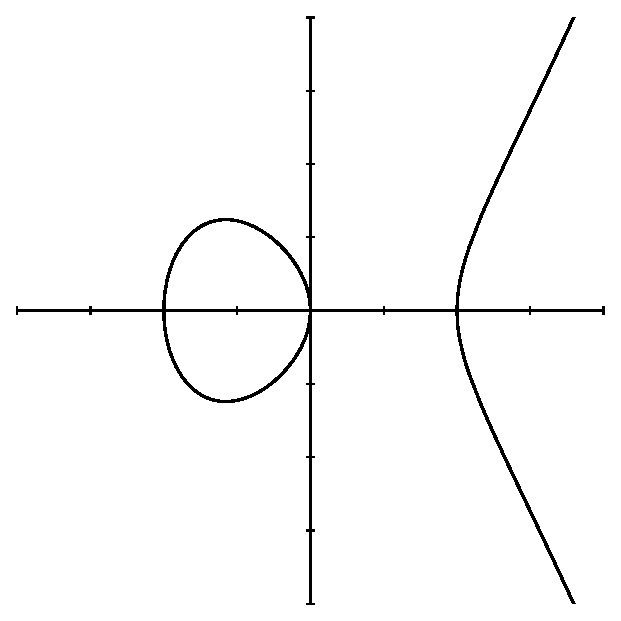
\includegraphics{x3-xa}}
  \put(-90,150){\line(4,1){260}}
  \put(83,230){\line(0,-1){220}}
  \put(-84,160){$P_1$}
  \put(-71,155){\circle*{4}}
  \put(-20,180){$P_2$}
  \put(-13,169){\circle*{4}}
  \put(58,200){$-P_3$}
  \put(83,193){\circle*{4}}
  \put(89,92){$P_3 = P_1 + P_2$}
  \put(83,90){\circle*{4}}
 \end{picture} 
\end{center}
\caption{Addition on the curve $y^2 = x^3 - x$\label{Elliptic:Addition:Fig}}
\end{figure}

The additive structure of points on an elliptic curve can also be
given an intuitive geometric interpretation.  An elliptic curve is
represented by a polynomial of degree $3$, which we assume to be in
Weierstrass form:
\[
y^3 = x^3 + ax + b.
\]
\figref{Elliptic:Addition:Fig} shows a sample curve in this form. 

In general a straight line will intersect a cubic curve at three
points.  We define the sum of three three co-linear points on an
elliptic curve to be zero. This definition preserves the symmetry of
the three points.

Notice that a vertical line only intersects an elliptic curve of this
form at two finite points.  Its third intersection point is at
infinity.  The zero of the group of points on an elliptic curve is
defined to be this point at infinity.

Thus the sum of two points $P_1$ and $P_2$ on an elliptic curve can be
computed as illustrated in \figref{Elliptic:Addition:Fig}.  A line is
draw through $P_1$ and $P_2$.  This line will intersect the elliptic
curve at a third point $-(P_1+P_2)$.  A vertical line is draw through
$-(P_1+P_2)$ which will intersect the curve at $P_1+P_2$.

\subsection{Algebraic Addition Formula}
\label{Elliptic:Alg:Add:Sec}

For computational purposes it is convenient to use a slightly different
form of the equation for the curve.  From here on we use:
\begin{equation} \label{El:WeierForm:Eq}
E : y^2 = x^3 + a x + b.
\end{equation}
Notice that we have removed the factor of $4$ that proceeded the cubic
term in \eqnref{Weier:DE:Eq}.  This is in keeping with the algebraic
formulation of the elliptic curve.  The $\wp$-function parameterizes a
point $P_1 = (x_1, y_1)$ on the curve as
\[
(x_1, y_1) = (\wp(u_1), \frac{\wp'(u_1)}{2}).
\]
Let $P_2 = (x_2, y_2)$ be a second point on the curve elliptic curve
$E$, with its own parameter $u_2$.  The addition formulas for $\wp$,
(\ref{WeierAddition:Eqa})--(\ref{WeierDouble:Eqb}), provides a third
point on $E$, $P_3 = (x_3, y_3)$, whose parameter is $u_1 + u_2$.
Its coordinates are
\[
\begin{aligned}
x_3 &= - x_1 - x_2 + m^2 \\
y_3 &= - y_1 + (x_1 - x_3) m
\end{aligned}
\]
where
\[
m = 
  \begin{cases}
    \displaystyle \frac{y_2 - y_1}{x_2 - x_1}& \mbox{when $P_1 \not= P_2$;}\\
    \displaystyle \frac{3 x_1^2 + a}{2 y_1}  & \mbox{when $P_1 = P_2$.}
  \end{cases}
\]
$P_3$ is the sum of $P_1$ and $P_2$ on the elliptic curve $E$.  

$P_3$ is the point at infinity (the zero element of $E$) when the
denominators of its coefficients go to zero.  When $P_1 \not= P_2$
this occurs when $x_1 = x_2$.  So two points on $E$ that lie on a
vertical line are additive inverses of each, just as suggested by the
geometric discussion.   

For the case $P_1 = P_2$, assume that the characteristic of the ground
field is not $2$.  In this case $P_1$ has order $2$, \ie, $2P_1 = 0$,
which can only occur when $y_1 = 0$.  Factoring the right hand side of
\eqnref{El:WeierForm:Eq} gives
\[
y^2 = (x - \lambda_1) (x - \lambda_2) (x - \lambda_3).
\]
The only points on $E$ which have order $2$ are $(0, \lambda_1)$, $(0,
\lambda_2)$ and $(0, \lambda_3)$.  As can be seen from
\figref{Elliptic:Addition:Fig} these points have vertical tangents as
expected.

\subsection{Hessian Form of Curve}
\label{Elliptic:Hessian:Add:Sec}

There are other formulations of elliptic curves that that can be
especially useful for computations.  This section gives the Hessian
form of the elliptic curve which was suggested in\cite{Chudnovsky85}.
The primary advantage of this form of the elliptic curve is that the
resulting addition formulas do not require the computation of an
inverse.

The Hessian form of the elliptic curve is most naturally discussed in
projective space,\index{projective space} $\P^2$.  Recall that points
in the two dimension projective space over $k$, $\P^2(k)$, consists of
triples $x,y,z \in k$, not all of which are zero, where two triples
are considered equivalent if there exists an $r \in k$ such that
\[
(x_1, y_1, z_1) = (r x_2, r y_2, r z_2).
\]
The equivalence class of points in $\P^2(k)$ that contains $(x, y, z)$
is denoted by $(x:y:z)$.

Unlike the Weierstrass model, the Hessian model of the elliptic curve
has only a single parameter:
\[
x^3 + y^3 + z^3 = D x y z.
\]
If $P_1 = (x_1, y_1, z_1)$ is a point on the cubic in Hessian model, then its
inverse is $-P_1 = (y_1, -x_1, z_1)$.  The identity of the group is the
point $(1, -1, 0)$.  Let $P_3$ be inverse of the sum of the two points
$P_1$ and  $P_2$, \ie{} $P_1 + P_2 + P_3 = 0$.  Then we have
\begin{eqnarray*}
x_3 &= &x_1^2 y_2 z_2 - x_2^2 y_1 z_1
= (x_1 y_2) \cdot (x_1 y_2) - (x_2 z_1) \cdot (x_2 y_1), \\
y_3 &= &x_2 y_1^2 z_2 - x_1 y_2^2 z_1
= (y_1 z_2) \cdot (x_2 y_1) - (x_1 y_2) \cdot (y_2 z_1), \\
z_3 &= &x_2 y_2 z_1^2 - x_1 y_1 z_2^2
= (x_1 z_1) \cdot (y_2 z_1) - (x_1 z_2) \cdot (y_1 z_2),
\end{eqnarray*}
if $P_1 \not= P_2$.  The second formulation given above minimizes the
number of multiplications required.  If $P_1 = P_2$ the the following
formulae can be used
\begin{eqnarray*}
x_3 & = & x_1(y_1^3 - z_1^3), \\
y_3 & = & y_1(z_1^3 - x_1^3), \\
z_3 & = & z_1(x_1^3 - y_1^3). 
\end{eqnarray*}
This model has the added advantage that it is particularly easy to pick
a curve and point on the curve.  Picking a point $(x_1, y_1, z_1)$
automatically choses an elliptic curve with invariant 
\[
D = \frac{x_1^3 + y_1^3 + z_1^3}{x_1 y_1 z_1}.
\]

\section{Endomorphisms of Elliptic Curves}
\label{Elliptic:Endo:Sec}

Using any of the forms of addition laws for an elliptic curve $E/k$
discussed in the previous section, the points of $E$ form an abelian
group.  We denote by $E(k)$ the points of $E$ whose coordinates lie in
$k$.  This is sometimes abbreviated as $E$ when $k$ is understood.  In
general we will be interested in $E(\bar{k})$ where $\bar{k}$ is the
algebraic closure of $k$.  This section discusses the endomorphisms of
$E(\bar{k})$, \ie{} the set of group homomorphisms of $E(\bar{k})$
into $E(\bar{k})$.

Let $\lambda_1$ and $\lambda_2$ be two endomorphisms of this group,
and $P \in E$, $\lambda_1(P)$ and $\lambda_2(P)$ are elements of $E$.
The sum of $\lambda_1$ and $\lambda_2$ is defined to be the
endomorphism
\[
P \mapsto \lambda_1(P) + \lambda_2(P),
\]
and the product $\lambda_1 \lambda_2$ by
\[
P \mapsto \lambda_1 (\lambda_2(P)).
\]
We will denote this ring, called the {\em endomorphism ring of
$E$}\index{elliptic curve!endomorphism ring} by $\End
E$.\addsymbol{$\End E$}{Ring of endomorphisms of an elliptic curve,
$E$.} If the points on $E$ are restricted to have coordinates in a
field $k$ we will denote the ring of endomorphisms by $\End_k E$.

We associate the rational integers with elements of $\End E$ as follows:
\[
n : P \mapsto [n]\circ P = \overbrace{P + P + \cdots + P}^{n}.
\]
Coupled with the fact that $E$ is a group so for every $P \in E$ there
is a point $-P$, this provides a map $\Z \rightarrow \End E$.

To illustrate this, consider the effect of $[2]$ on elements of $E: y^2 =
x^3 + ax +b$.  Let $P = (x, y)$ be generic point of $E$.  Then
\[
P+ P = ( -2x +m^2, -y + (3x -m^2) m),
\]
where 
\[
m = \frac{3x^2+a}{2y} \quad\mbox{and}\quad
m^2 = \frac{9x^4+6ax^2 +a^2}{4(x^3 +ax+b)},
\]
where we have used $y^2 = x^3+ax+b$ to eliminate the $y^2$ term.
This gives,
\begin{equation}\label{El:Double:Eq}
[2]\circ P = \left( \frac{x^4-2ax^2-8bx+a^2}{4(x^3+ax+b)}, 
   \frac{x^6+5ax^4+20bx^3-5a^2x^2-4ab-8b^2-a^3}{8(x^3+ax+b)y}\right).
\end{equation}
That $[2]$ is an endomorphism of $E$ can be seen by computing
\[
\begin{aligned}
\frac{x^4-2ax^2-8bx+a^2}{4(x^3+ax+b)}^3 &+ a
\frac{x^4-2ax^2-8bx+a^2}{4(x^3+ax+b)} +b \\
&= \frac{(x^6+5ax^4+20bx^3-5a^2x^2-4ab-8b^2-a^3)^2}{64(x^3+ax+b)^3} \\
&=
\left(\frac{x^6+5ax^4+20bx^3-5a^2x^2-4ab-8b^2-a^3}{8(x^3+ax+b)y}\right)^2.
\end{aligned}
\]

Hand computations for larger values of $n$ are quite cumbersome.
Nonetheless, the mathematicians of th 19\th{} century developed the
following set of fascinating formulas for computing $[n]$.  Define
$\Psi(x,y)$ as 
\[
\Psi_{-1}(x,y) = -1, \quad \Psi_{0}(x,y) = 0, \quad
\Psi_{1}(x,y) = 1, \quad
\Psi_{2}(x,y) = 2y,
\]
\[
\Psi_3(x,y) = 3 x^4 + 6a x^2 + 12 b x - a^2,
\]
\[
\Psi_4(x,y) = 4y(x^6 + 5a x64 + 20bx^3 - 5a^2 x^2 - 4abx -8b^2-a^3).
\]
For larger values of $n$ $\Psi_n$ satisfies the following recurrence
relations 
\[
\begin{aligned}
\Psi_{2n}(x,y) &= \displaystyle {\frac{\Psi_n}{2 y}}
\left(\Psi_{n+2} \Psi_{n-1}^2 - \Psi_{n-2} \Psi_{n+1}^2\right),\\
\Psi_{2n+1} &= \Psi_{n+2} \Psi_n^3 - \Psi_{n+1}^3 \Psi_{n-1}.
\end{aligned}
\]

Since we are only concerned with values on $E$ we can replace $y^2$
wherever it occurs by $x^3 +ax+b$.  By induction, we can show that 
$\Psi_{2n+1}$ is free of $y$, while $\Psi_{2n} \in y k[x]$.  Let
$f_n$ be the $\Psi_n$ when $n$ is even and $\Psi_n/y$ when $n$ is odd.
Again by induction we easily get:

\begin{proposition}
The degree of $f_n$, when $p$ does not divide $n$, is
\[
\deg f_n = 
  \begin{cases}
    \frac{1}{2}(n^2 -1), & \mbox{if $n$ is odd;} \\ %\noalign{\vskip3pt}
    \frac{1}{2}(n^2-4).  & \mbox{if $n$ is even.}
  \end{cases}
\]
\end{proposition}

The crucial property of these polynomials is that they can be used to
compute the effect $[n]$.

\begin{proposition}\label{Ell:nMult:Prop}
Let $P= (x, y)$ be a point on the elliptic curve $E$
that does not have $n$-torsion.  Then
\[
nP = \left(x - \frac{\Psi_{n-1} \Psi_{n+1}}{\Psi_n^2},
\frac{\Psi_{n+2} \Psi_{n-1}^2 - \Psi_{n-2} \Psi_{n+1}^2}{4y \Psi_n^3}\right).
\]
\end{proposition}

With a moderate amount of effort, this proposition can be proved by
induction. 

Most of the elements in the group of points of an elliptic curve have
infinite order.  Some points, however, have finite order.  That is the
point $P$ has order $\ell$ when $\ell P = O_E$.  The set of all points
in $E$ that have finite order is a subgroup of $E$ called the
\keyi{torsion subgroup} of $E$.

Examining the formula given above for $nP$, we see that the $nP$ is
the identity (in $E$) when $\Psi_n = 0$, or equivalently when $f_n(x)
= 0$.  We state this as the following proposition.

\begin{proposition} \label{TorsionCriteria:Prop} 
Let $P = (x, y)$ be a point on the elliptic curve $E$ that is not of
order $2$.  Then $P$ has $n$ torsion if and only if $f_n(x)=0$.
\end{proposition}

The torsion subgroup of an elliptic curve over $\Q$ is finite.
{\Mazur} has proven the following remarkable theorem about the
structure of torsion subgroup of $E(\Q)$ \cite{Mazur77,Mazur78}.

\begin{proposition}[{\Mazur}]
The torsion subgroup of $E$, an elliptic curve defined over $\Q$, is
isomorphic to one of the following: $\Z/m\Z$ for $m\le 10$ or $m=12$,
or $\Z//2\Z \oplus \Z/m\Z$ for $m\le 4$.
\end{proposition}

\medskip
For many elliptic curves, the ring of endomorphisms is just $\Z$.
However, sometimes it is larger.  These special cases are called
elliptic curves with {\em complex multiplication} for reasons that
will be clear shortly. 

To get an intuitive understanding of the structure of $\End E$, we
return to the analytic view of elliptic curves.  First notice that the
embedding of $\Z$ in $\End E$ means that for each $n$, positive or
negative, $\wp(nz)$ can be written as a rational function in terms of
$\wp(z)$ and $\wp'(z)$.  Sometimes there are numbers outside of $\Z$
that also have this property.

An endomorphism $\lambda \in \End_{\C} E$ maps $\C/L$ into itself.
Thus it must map $C$ into itself preserving the additive group
structure of $\C$, and consequently must be multiplication by a
constant.  Furthermore, $\lambda$ must map the lattice into itself.
The largest ring that always satisfies this last requirement is the
rational integers $\Z$.  Thus $\Z$ is always a subring of $\End_{\C}
E$, which we just demonstrated.  If the endomorphism ring contains
elements other than $\Z$, then $E$ is said to admit \keyi{complex
multiplications}.  If there is an element of $\End_{\C}$, $z$, that is
not a rational integer, then $E$ is said to admit {\em complex
multiplication by $z$\/}.\index{elliptic curve!complex multiplication} 

For simplicity, assume that the basis for the lattice $L$ is 
$(1, \omega)$, and assume that the curve $E$ admits complex multiplication
by $z$.  Then $z$ must map each element of $L$ into $L$; in particular
it must send the basis elements into $L$.  Thus,
\begin{eqnarray*}
z\cdot 1 &=& a + b \omega,\\
z \cdot \omega &=& c + d \omega,
\end{eqnarray*}
where $a$, $b$, $c$ and $d$ are all rational integers.
The first equations shows that $z$ must be an element of $L$.
Combining these two equations gives
\[
(a + b \omega) \omega = c + d \omega.
\]
Thus $\omega$ must be a complex quadratic number, as must $z$.  

When the elliptic curve admits complex multiplication by $\omega$,
$\wp(\omega z)$ is a rational function in $\wp(z)$ and $\wp'(z)$.
This is somewhat surprising.  Returning to the purely algebraic
framework, consider the elliptic curve $E : y^2 = x^3 - x$.
If $P = (x, y)$ is a generic point on $E$, then using \eqnref{El:Double:Eq}
\[
[2] : (x, y) \mapsto
\left( \frac{x^4+2ax^2+1}{4(x^3-x)}, 
   \frac{x^6-5x^4-5x^2+1}{8(x^3-x)y}\right).
\]
From the geometric construction it is clear that
\[
[-1] : (x, y) \mapsto (x, -y),
\]
which can also be verified algebraically. 

This particular curve also admits a complex multiplication by $i$.
The map 
\[
[i] : (x, y) \mapsto (-x, iy)
\]
is an endomorphism of $y^2 = x^3 -x$.  Clearly, $[i] \circ [i] =
[-1]$.  Using the additional formula given above, we can compute the
endomorphism $[1+i]$:
\[
[1+i] : (x, y) \mapsto \left(-\frac{i}{2}\left(x - \frac{1}{x}\right),
  -\frac{1+i}{4}\left(1 + \frac{1}{x^2}\right) y\right).
\]
Composing $[1+i]$ with itself we have
\[
\begin{aligned}
[1+i]\circ[1+i](x,y) & = \left(
-\frac{x^4+2x^2+1}{4x^3-4x}, \frac{i(x^6-5x^4-5x^2+1)}{8(x^3-x)^2}y\right)\\
& = [i] \circ [2] (x,y).
\end{aligned}
\]
In fact, the endomorphism ring of $y^2=x^3-x$ is isomorphic to $\Z[i]$.

\medskip
There is an additional endomorphism of an elliptic curve over a
finite field of characteristic $p$.  Let $E(\bar{\F}_q)$ be the group
of points over $\bar{\F}_q$ of the elliptic curve $E/\F_q$.  Then the map
\[
\phi_{p^{\ell}} : (x, y) \mapsto (x^{p^{\ell}}, y^{p^{\ell}})
\]
is an endomorphism of $E$ called the \keyi{Frobenius morphism}.  From
the discussion of complex multiplication for an elliptic curve over
$\C$, we expect that $\phi$ would either be the same as multiplication
by an integer or would be the solution of a quadratic equation.

\section{Zeta Functions and the Riemann Hypothesis}
\label{Elliptic:Zeta:Sec}

Let $E/\F_p$ be an elliptic curve over $\F_p$ and denote by $N_k$ the
number of points on $E$ over $\F_{p^k}$ counting the points at
infinity.  The affine plane over $\F_{p^k}$ has $p^{2k}$ points, while
the hyperplane at infinity has $p^k$ points, so the number possible
points in the projective plane over $\F_{p^k}$ is $p^k(p^k+1)$.  Lying
on the elliptic curve provides one polynomial constraint on the
coefficients, so we would expect there to be about $p^k$ points on
$E$.

The \keyi{zeta function} of the elliptic curve $E$ is defined to be 
\[
Z_E(u) = \exp \sum_{k=1}^{\infty} \frac{N_k}{k} u^k .
\]
Writing it in the form $\zeta_{E,p}(s) = Z_E(p^{-s})$ we can see its
relation with Riemann zeta function $\zeta(s)$.  Taking the logarithm
derivative of $\zeta_{E,p}(s)$ we get
\[
\frac{\zeta_{E,p}'(s)}{\zeta_{E,p}(s)} =
- \sum_{k=1}^{\infty} \frac{N_k \log p}{p^{ks}}.
\]
Taking the logarithmic derivative of the Euler product of the Riemann
zeta function () we have
\[
 \frac{\zeta'(s)}{\zeta(s)} 
     = \frac{d}{ds} \log \prod_p \left(1 - p^{-s}\right)^{-1}
     = -\sum_p \log p \frac{p^{-s}}{1 - p^{-s}}.
\]
Expanding each term as a power series in $p^{-s}$ we have
\[
\frac{\zeta'(s)}{\zeta(s)} 
  = - \sum_p \sum_{k=1}^{\infty} \frac{\log p}{p^{ks}}.
\]
Factoring $\zeta(s)$ into $\prod_p \zeta_p(s)$ we have
\[
\zeta_p(s) = - \sum_{k=1}^{\infty} \frac{\log p}{p^{ks}},
\]
which corresponds precisely with the $\zeta_{E,p}(s)$.

The zeta function of an elliptic curve shares a number of fundamental
properties with the Riemann zeta function.  In 1949 {\Weil} stated
these properties in enormous generality, extending far beyond elliptic
curves.  The final piece of the {\Weil}'s program was given by
{\Deligne} in 1974.  The following proposition gives {\Weil}'s basic
statements for the special case of a elliptic curve.

\begin{proposition} \label{Ell:Weil:Conject:Prop}
Let $E/\F_q$ be an elliptic curve and $Z_E(u)$ its zeta function.
Then $Z_E$ satisfies the functional equation
\[
Z_E(\frac{1}{q u}) =  Z_E(u).
\]
and $Z_E$ has the form
\[
Z_E(u) = \frac{(1 - \alpha_1 u) (1 - \alpha_2 u)}{(1 - u)(1 - q u)},
\]
where the $|\alpha_i| = q^{1/2}$.  Furthermore, $\alpha_1 \alpha_2$
and $\alpha_1 + \alpha_2$ are rational numbers.
\end{proposition}

If these statements are converted to statements about $\zeta_{E,p}(s)$
they take the form more familiar from the Riemann zeta function.  The
functional equation is
\[
\zeta_{E,q}(1 - s) = \zeta_{E,q}(s)
\]
while second statement claims 
\[
\zeta_{E,q} = \frac{(1 - \alpha q^{-s}) (1 - \beta q^{-s})}{(1 - q^{-s})(1 - q^{1-s})}.
\]
$|\alpha_i| = q^{1/2}$ means that the zeroes of $Z_E(u)$ have
absolute value $q^{-1/2}$.  Thus the zeroes of $\zeta_{E,q}(s) =
\zeta_E(q^{-s})$ have real part = $1/2$.

\section{Calculation of $N_p(E)$}
\label{Elliptic:Order:Sec}

By the analysis of the previous section, we have seen that the number
of points in $E(\F_q)$ is intimately tied to the \keyi{Frobenius
element}.  In particular 
\[
N_q(E) = \#E(\F_q) = q + 1 - \Tr \phi_q.
\]
Thus the key problem in determining the order of the group is to
compute the trace of the Frobenius endomorphism.  We know that in the
ring of endomorphisms of $E$ the Frobenius element satisfies
\[
\phi_q^2 - t \phi_q + q = 0.
\]
That is, the endomorphism $\phi_q^2 - t \phi_q + q$ sends all of the
elements of $E$ to zero.  So, for a generic point $(x,y) \in E$
\begin{equation} \label{Ell:Trace:Null:Eq}
\begin{aligned}
[\phi_q^2 - t \phi_q + q] \circ (x, y) 
  & = (x^{q^2}, y^{q^2}) - [t]\circ(x^q, y^q) + [q] \circ (x, y), \\
  & = 0_E.
\end{aligned}
\end{equation}
Remember that multiplication by a specific integer can be computed by
\propref{Ell:nMult:Prop} or by repeated squaring.

One way to determine $t$ would be to evaluate
\eqnref{Ell:Trace:Null:Eq} for $t=0, 1, -1, 2, -2, \ldots$ until it
vanished.  Unfortunately this leads to an algorithm of time complexity
approximate $O(q^{1/2})$ since $|t| < 2\sqrt{q}$ by the Riemann
hypothesis (\propref{Ell:Weil:Conject:Prop}).  Instead we use the the
Chinese remainder theorem so that we will only need to evaluate
\eqnref{Ell:Trace:Null:Eq} for $O(\log q)$ different values of $t$.

Let $E[\ell]$ denote those elements of $E$ whose order divides $\ell$.
By \propref{TorsionCriteria:Prop} if $(x,y) \in E[\ell]$ then
$f_{\ell}(x)$ vanishes.  For any such element, notice that there is
no difference between the action of $[n]$ and $[n+\ell]$.  
Restricting the endomorphisms of  $E$ to the elements of $E[\ell]$
maps the elements of $\Z$ in $\End E$ to elements of $\Z/\ell\Z$.

So in $\End E[\ell]$, $t$ is sent to its image modulo $\ell$,
$t_{\ell}$. To determine if $t \equiv 0 \pmod{\ell}$, compute
\[
(x^{q^2}, y^{q^2}) + [q]\circ(x,y) = 
(x^{q^2}, y^{q^2}) + \left(x - \frac{\Psi_{q-1} \Psi_{q+1}}{\Psi_q^2},
\frac{\Psi_{q+2} \Psi_{q-1}^2 - \Psi_{q-2} \Psi_{q+1}^2}{4y
\Psi_q^3}\right)
\]
modulo $f_{\ell}(x)$.  If we get $O_E$, then $t_{\ell} = 0$.  

To determine $t_{\ell}$ we compute $\phi_q^2 - s \phi_q + q$ for $s =
0, \ldots, \ell -1$.  When this expression gives zero, $t_{\ell} = s$.
This approach for computing $N_p(E)$ is due to {\Schoof} \cite{Schoof:SQRT}.

Careful analysis of this techniques shows that approximately $O(\log^9
p)$ operations are required to compute $\Tr \phi$.

This technique should be implemented using the Hessian formulation of
the elliptic curve.  Testing if we've generated $O_E$ will be easier
than with Schoof's approach and and the computations should be faster
(and more parallelizable) since there is no division to slow things
down.  You can't use the division formulas anymore, but computing $nP$
by repeated addition should be just as fast.


\section{Modular Invariant}

Two elliptic curves are equivalent if there is .... \Marginpar{need more
here}  The {\em $j$-invariant} of an elliptic curve is a quantity that
identifies the equivalence class, to which the curve belongs.  It is
defined as
\[
j = \frac{g_2^3}{g_2^3 - 27g_3^2}.
\]

\section*{Notes}

\footnotesize

A more thorough discussion of elliptic
curves can be found in {\Tate}'s paper \cite{Tate74} and the books
by {\Koblitz} \cite{Koblitz:Elliptic}, {\Lang} \cite{Lang:Elliptic} and
{\Silverman} \cite{SilvermanJH86}.

\normalsize
